
\section{Design of \sys}

\begin{figure*}[!h]
    \centering
    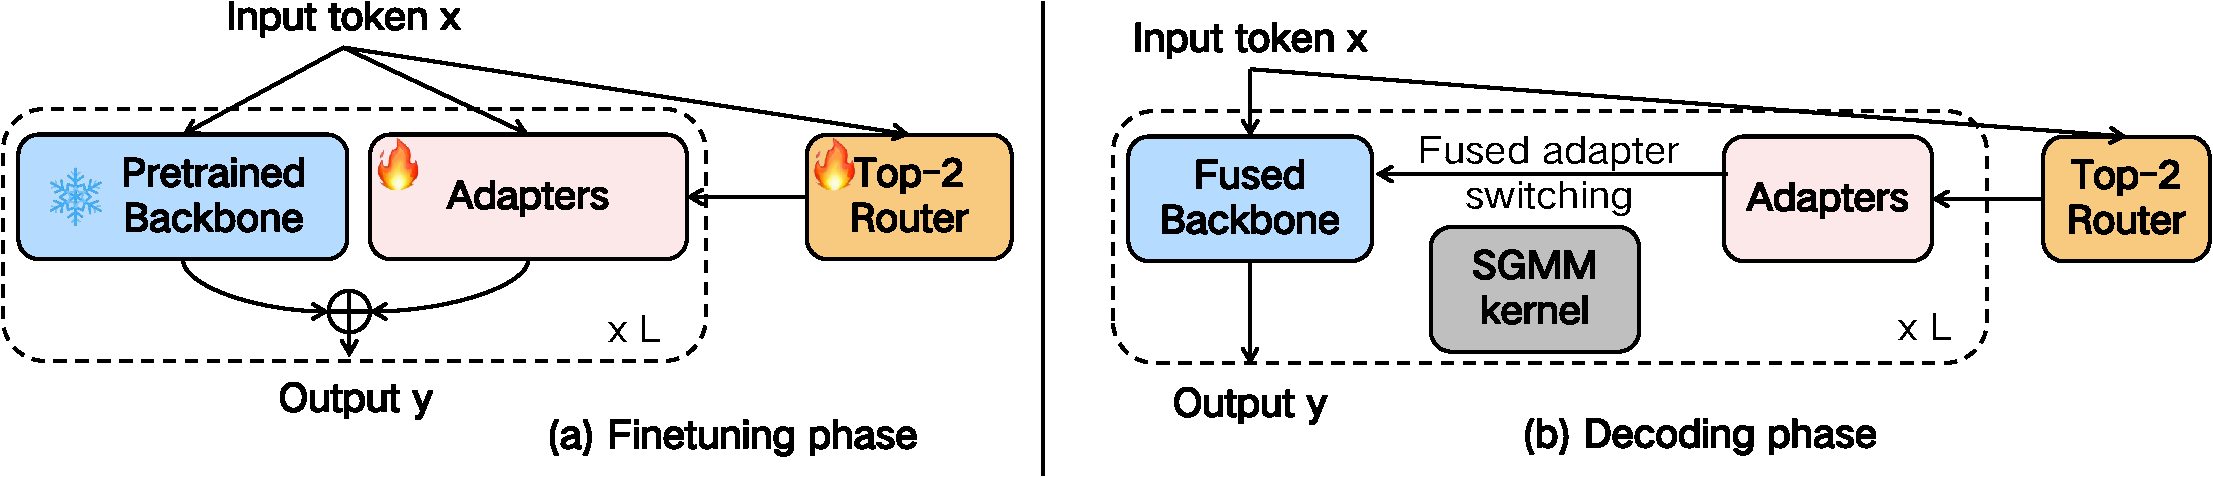
\includegraphics[width=1\linewidth]{figures/overview.pdf}
    \caption{Overview of \sys.}
    \label{fig:overview}
\end{figure*}

\subsection{Overview}

As shown in Figure~\ref{fig:overview}, given a pre-trained LLM, we first extend it with \sys to enhance its model capacity and then finetune it on either general or domain-specific datasets. 
The core innovation of \sys lies in its token-wise pre-gated architecture, which fundamentally differs from existing layer-wise or block-wise dynamic adapter approaches. Instead of making routing decisions at each layer independently, \sys employs a single router at the first layer to determine expert activation patterns for all subsequent layers, thereby eliminating the computational overhead of repeated routing computations.

During the decoding phase, each token is initially processed through a router to compute the gating for each layer. The key insight is that once we determine which experts should be activated for a given token, this decision can be propagated across all layers without requiring additional routing computations. This design choice is motivated by our observation that tokens with similar semantic properties tend to activate consistent expert patterns across different layers.
% 
To implement this efficiently, we developed an SGMM kernel that facilitates fast fused adapter switching. This advanced functionality enables the rapid merging of activated adapters into the backbone and the efficient unmerging of inactivated adapters from the backbone, significantly reducing the number of CUDA kernel calls.

\subsection{Model Structure} \label{section:method:structure}

In \sys, we extend adapters only in the linear layers of the pre-trained backbone, and we insert a Top-2 router $G^1$ only at the first expanded linear layer. This architectural choice is carefully designed to balance computational efficiency and model expressiveness.

\noindent\textbf{Router Architecture.} The Top-2 router $G^1$ consists of a lightweight linear transformation followed by a softmax activation and top-k selection mechanism. The router takes the hidden representation from the first layer as input and produces routing weights that determine expert activation across all layers.

\noindent\textbf{Expert Configuration.} Each expert in \sys is implemented as a LoRA module with rank $r$ typically set to 64 or 128, depending on the model size and task complexity. The number of experts $N$ is configurable and typically ranges from 4 to 16, providing a good balance between model capacity and computational overhead.

\noindent\textbf{Finetuning Phase.}
As shown in Figure~\ref{fig:overview} (a), during fine-tuning, the computation process can be written as:
\begin{equation}
    y^l = f^l(x^l) + \sum_{i = 1}^{N}{G^1(x^{1})_iE^l_i(x^l)}
    \label{equation:ours:definition}
\end{equation}
where \sys only replaces the $G^l(x^l)$ with $G^1(x^{1})$ in Equation~\ref{eq:moa_origin}, where $x^{1}$ denotes the input in the first expanded linear layer. \sys employs a token-wise pre-gated LoRA structure, meaning that the routing weights for all layer adapters are identical. 
This design not only preserves the model's dynamicity but also facilitates latency optimization during inference.

\noindent\textbf{Decoding Phase.}
As depicted in Figure~\ref{fig:overview} (b), \sys leverages the token-wise pre-gated structure to reduce latency during the decoding phase. During the decoding phase of LLM generation, where the input \( x \) is a single token, the Top-2 router $G^1$ determines which experts' adapters are activated. 
Then the activated experts are merged into pretrained backbone. Finally, the fused backbone performs forward process and the decoding computation as:
\begin{align}\label{equation:ours:1}
    y^l = f^l_*(x^l)
\end{align}
To efficiently calculate $f^l_*$ for all layers, we propose to perform fused adapter switching with the SGMM kernel, which merges the parameters of all activated expert adapters across all layers into the original parameters of the pretrained model in a single CUDA kernel operation. 
Finally, the fused backbone execute just like the initial pretrained backbone as shown in Equation~\ref{equation:ours:1}.

\noindent\textbf{Prefilling Phase.}
The latency of \sys during the prefilling phase is comparable to that of existing dynamic adapters. For the prefilling phase, we have not implemented specific optimizations, as the latency in the LLM generation stage primarily originates from the decoding phase.

\subsection{Fused Adapter Switching}    \label{section:method:switching}
To calculate $f^l_* = f^l + \sum_{i = 1}^{N}{G^1(x^1)_i} E^l_i$ according to Equation~\ref{eq:moa_origin} and Equation~\ref{equation:ours:definition}, we may merge multiple experts adapters into backbone because one input token may activate multiple adapters (typically Top-2). The experts in \sys are LoRA adapters, which contain down projection \text{LoRA\_DOWN} and up projection \text{LoRA\_UP}.

We only need to invoke the CUDA kernel $k$ times instead of $N$ times, as $G^1(x^1)$ specifically targets the top-$k$ selections. To further reduce the number of CUDA kernel calls, we concatenate all LoRA adapters before merging them into the original model parameters as:
\begin{flalign}\label{equation:ours:lora_unified_single}
    &\text{LoRA\_DOWN}^l = \text{concat}\big[G^1(x^1)_i \cdot \text{LoRA\_DOWN}^l_i, \nonumber \\
    &\hfill i=1,\ldots,N\big] & \\
    &\text{LoRA\_UP}^l = \text{concat}\big[\text{LoRA\_UP}^l_i, i=1,\ldots,N\big] &
\end{flalign}

Thus, we can merge the concatenated LoRA adapters into origin backbone as:
\begin{align}\label{equation:ours:lora merge2}
    f^l_* = f^l + \text{LoRA\_DOWN}^l \times \text{LoRA\_UP}^l
\end{align}

We observe that during the decoding phase, the activated adapters varying from one token to the next. A simple way to obtain $f^l$ is to unmerge the activated adapters by the last token in the current iteration. Then we concatenate the activated adapters of current input and inactivated adapters of last input as:
% \begin{align}\label{equation:ours:lora unified fused}
%     \text{Fused\_LoRA\_DOWN}^l &= \text{concat}([-(\text{LoRA\_DOWN}^l)^{t-1}, \nonumber \\
%     &\qquad (\text{LoRA\_DOWN}^l)^{t}]) \\
%     \text{Fused\_LoRA\_UP}^l &= \text{concat}([(\text{LoRA\_UP}^l)^{t-1}, \nonumber \\
%     &\qquad (\text{LoRA\_UP}^l)^{t}])
% \end{align}
\begin{align}\label{equation:ours:lora_unified_fused}
    &\text{Fused\_LoRA\_DOWN}^l = \text{concat}\big[-(\text{LoRA\_DOWN}^l)^{t-1}, \nonumber \\
    &\hfill (\text{LoRA\_DOWN}^l)^{t}\big] \\
     &\text{Fused\_LoRA\_DOWN}^l = \text{concat}\big[-(\text{LoRA\_DOWN}^l)^{t-1}, \nonumber \\
    &\hfill (\text{LoRA\_DOWN}^l)^{t}\big]   
\end{align}


So the concatenated LoRA adapter switching operation can be rewritten as:
% \begin{align}\label{equation:ours:fused}
%     (f^l_*)^t &= (f^l_*)^{t-1} + \text{Fused\_LoRA\_DOWN}^l \times \text{Fused\_LoRA\_UP}^l
% \end{align}

\begin{equation}\label{equation:ours:fused}
\begin{split}
    (f^l_*)^t &= (f^l_*)^{t-1} + \quad \text{Fused\_LoRA\_DOWN}^l \times \\ &\text{Fused\_LoRA\_UP}^l
\end{split}
\end{equation}

To calculate Equation~\ref{equation:ours:fused}, we utilize our efficiently designed CUDA kernel, SGMM, to seamlessly integrate these fused adapters into the pretrained LLM backbone for all layers with only one CUDA kernel call.

\subsection{SGMM Kernel}    \label{section:method:sgmm}

The straight-forward way to merge the LoRA adapter into the backbone is to merge them layer by layer. This approach requires multiple calls to the CUDA kernel, which introduces additional latency due to kernel launches. Moreover, smaller kernel computations underutilize GPU thread blocks, leading to a low GPU throughput. We observe the layer-by-layer merging operations can be handled concurrently and introduce a CUDA kernel called Segmented Gather Matrix Multiplication (SGMM) to finally handle the merging of LoRA adapters of \sys, adapted from the concept of SGMV proposed by Punica \cite{chen2023punica}.

SGMM is designed to execute a batched GEMM operations, which can be summarized by the following equation:
\begin{equation}\label{equation:sgmm}
    f_* =  f +  \text{Fused\_LoRA\_DOWN} \times \text{Fused\_LoRA\_UP},
\end{equation}
where $f_*$ is the resultant updated matrix of the backbone; $f$ is the original weight matrix of the backbone; $\text{Fused\_LoRA\_DOWN}$ and $\text{Fused\_LoRA\_UP}$ are the adapter matrices for weight matrix $f$. The addition operation within the SGMM kernel is performed in place, significantly reducing the additional memory overhead.

When wrapping these operations into a single CUDA kernel, taking full advantage of the GPU's computational resources is challenging. To achieve this, we divide the matrix multiplication into multiple GEMM tiles and assign them to different thread blocks. On the other hand, these thread blocks must switch context with global memory/shared memory frequently, thus causing significant latency. To tackle this, we adopt a pre-fetch buffer mechanism to hide loading latency.

The input parameters for SGMM are arrays of pointers to the LoRA matrices and the backbone matrices, which respectively store the corresponding entries of each layer's LoRA matrix and the shape of each matrix segment. When launching the kernel, SGMM applies as many thread blocks as possible and divides the large matrix multiplication into multiple GEMM tiles of the same shape, with each tile operating matrix computation. The optimal tiling scheme related to hardware is selected to ensure the full utilization of each thread block. This parallel execution enables the efficient merging and unmerging of LoRA weights, a critical operation in our approach.

% Detailed implementation details of the SGMM kernel can be found in Appendix.
